\documentclass[12pt]{report}

%%%%%%%%%%%%%%%%%%%%%%%%
% Imports
%%%%%%%%%%%%%%%%%%%%%%%%
% \usepackage{minted} % Package for syntax highlighting (https://ctan.org/pkg/minted)
\usepackage[T1]{fontenc} % Standard package for selecting font encodings (https://ctan.org/pkg/fontenc)
\usepackage{color}
\usepackage{hyperref} % Extensive support for hypertext in LATEX (https://ctan.org/pkg/hyperref)
\usepackage{graphicx} % Enhanced support for graphics (https://ctan.org/pkg/graphicx). Should include EPS figures.
\usepackage{cite}
\usepackage{subfig}
\usepackage{geometry} % Change page size at any point
\usepackage[edges]{forest} % Drat tree like data structures (https://ctan.org/pkg/forest)
\usepackage{pgffor} % Loops in LaTeX (https://ctan.org/pkg/pgffor)
\usepackage{csvsimple} % Simple CSV file processing (https://ctan.org/pkg/csvsimple)
\usepackage{underscore} % Control the behaviour of "_" in text (https://ctan.org/pkg/underscore)
\usepackage{listings} % Typeset source code listings using LATEX (https://ctan.org/pkg/listings)
\usepackage[title]{appendix}
\usepackage{adjustbox}
\usepackage{tikz}
\usepackage{xspace}
\usepackage{wrapfig}
\usepackage{amsmath}

%%%%%%%%%%%%%%%%%%%%%%%%
% Settings
%%%%%%%%%%%%%%%%%%%%%%%%
% \addto\extrasenglish{%
%     \providecommand*{\lstlistingautorefname}{List.}
%     % \renewcommand*{\listingscaption}{Code}
%     \renewcommand*{\equationautorefname}{Eq.}
%     \renewcommand*{\figureautorefname}{Fig.}
%     \renewcommand*{\chapterautorefname}{Chap.}
%     \renewcommand*{\sectionautorefname}{Sec.}
%     \renewcommand*{\subsectionautorefname}{Sub-sez.}
% }
\renewcommand\UrlFont{\color{blue}\rmfamily} % Change URL font
\urlstyle{rm} % Change URL style

%%%%%%%%%%%%%%%%%%%%%%%%
% References
%%%%%%%%%%%%%%%%%%%%%%%%
% \addbibresource{resources.bib} %Import the bibliography file

%%%%%%%%%%%%%%%%%%%%%%%%
% Glossary
%%%%%%%%%%%%%%%%%%%%%%%%
% \makeglossaries
% \loadglsentries{glossary}

%%%%%%%%%%%%%%%%%%%%%%%%
% Minted
%%%%%%%%%%%%%%%%%%%%%%%%
% \setminted[solidity]{tabsize=2,breaklines,fontsize=\footnotesize}
% \setminted[typescript]{tabsize=2,breaklines,fontsize=\footnotesize}


%%%%%%%%%%%%%%%%%%%%%%%%
% Geometry
%%%%%%%%%%%%%%%%%%%%%%%%
\newcommand{\framedtext}[1]{%
\par%
\noindent\fbox{%
    \parbox{\dimexpr\linewidth-2\fboxsep-2\fboxrule}{#1}%
}%
}

%%%%%%%%%%%%%%%%%%%%%%%%
% Listings
%%%%%%%%%%%%%%%%%%%%%%%%
\definecolor{keywords}{HTML}{C586C0}
\definecolor{type}{HTML}{0000FF}
\definecolor{operator}{HTML}{569CD6}
\definecolor{comments}{HTML}{6a9955}
\definecolor{variable}{HTML}{9e9b00}
\definecolor{number}{HTML}{098658}
\definecolor{function}{HTML}{795E26}

\lstset{language=C++,
    basicstyle=\ttfamily\small,
    keywordstyle=\color{keywords}\ttfamily,
    stringstyle=\color{orange}\ttfamily,
    commentstyle=\color{comments}\ttfamily,
    morecomment=[l][\color{comments}]{\#}
}
\lstdefinelanguage{SMT2}{
    alsoletter=-, % Include dashes as letters
    sensitive=true,
    morekeywords={set-logic, declare-fun, assert, check-sat, get-model},
    morekeywords=[2]{Int, Bool, Real},
    morekeywords=[3]{and, or, not, imply, ite},
    morekeywords=[4]{a, b, c, d, e, f, g, h, i, j, k, l, m, n, o, p, q, r, s, t, u, v, w, x, y, z},
    morecomment=[l]{;},
    morestring=[b]",
}
\lstset{
    language=SMT2,
    basicstyle=\ttfamily\small,
    keywordstyle=\color{keywords},
    keywordstyle={[2]\color{type}},
    keywordstyle={[3]\color{operator}},
    keywordstyle={[4]\color{variable}},
    commentstyle=\color{comments},
    stringstyle=\color{orange},
    showstringspaces=false,
    tabsize=2,
    breaklines=true,
}
\lstdefinelanguage{mps}{
    alsoletter=-, % Include dashes as letters
    sensitive=true,
    morekeywords={NAME, ROWS, COLUMNS, RHS, RANGES, BOUNDS, BINARIES, GENERALS, ENDATA},
    morekeywords=[2]{N, L, E, G, UP, LO, FX, FR, MI, PL},
    morecomment=[l]{*},
    morestring=[b]",
}
\lstset{
    language=mps,
    basicstyle=\ttfamily\small,
    keywordstyle=\color{keywords},
    keywordstyle={[2]\color{type}},
    commentstyle=\color{comments},
    stringstyle=\color{orange},
    showstringspaces=false,
    tabsize=2,
    breaklines=true,
}
\lstdefinelanguage{bazel}{
    alsoletter=-, % Include dashes as letters
    sensitive=true,
    morekeywords={load, workspace, http_archive, cc_binary, cc_library, cc_test, cc_toolchain, cc_toolchain_suite, filegroup, genrule, package_group, package, sh_binary, sh_library, sh_test},
    morekeywords=[2]{glob},
    morecomment=[l]{\#},
    morestring=[b]",
}
\lstset{
    language=bazel,
    basicstyle=\ttfamily\small,
    keywordstyle=\color{keywords},
    keywordstyle={[2]\color{function}},
    commentstyle=\color{comments},
    stringstyle=\color{orange},
    showstringspaces=false,
    tabsize=2,
    breaklines=true,
}
\lstdefinelanguage{yacc}{
    alsoletter={\#, \%, -, _, :}, % Include dashes as letters
    morekeywords={\#include, \#define, \#ifdef, \#endif},
    morekeywords=[2]{% Bison keywords
            \%union, \%token, \%type, \%nonassoc, \%left, \%prec, \%right, \%start,
            \%grammar, \%pure_parser, \%define, \%expect, \%expect-rr, \%file, \%glr-parser,
            \%parse-param, \%parse-param-rr, \%skeleton, \%debug, \%output,
            \%locations, \%skeleton
        },
    morekeywords=[3]{% Bison variables
            , stringVal,
        }
    keywordstyle=\color{keywords}\bfseries,
    morecomment=[l][\color{comments}]{//}, % single-line comments
    morecomment=[s][\color{comments}]{/*}{*/}, % multi-line comments
    morestring=[b]",
    morestring=[b]',
}
\lstset{
    language=yacc,
    basicstyle=\ttfamily\small,
    keywordstyle=\color{keywords},
    keywordstyle={[2]\color{type}},
    keywordstyle={[3]\color{variable}},
    commentstyle=\color{comments},
    stringstyle=\color{orange},
    showstringspaces=false,
    tabsize=2,
    breaklines=true,
}
\lstdefinelanguage{flex}{
    alsoletter={\#, \%, -, _, :}, % Include dashes as letters
    morekeywords={\#include, \#define, \#ifdef, \#endif},
    morekeywords=[2]{% Bison keywords
            typedef
        },
    morekeywords=[3]{% Bison variables
            , stringVal,
        }
    keywordstyle=\color{keywords}\bfseries,
    morecomment=[l][\color{comments}]{//}, % single-line comments
    morecomment=[s][\color{comments}]{/***}{*/}, % multi-line comments
    morestring=[b]",
    morestring=[b]',
}
\lstset{
    language=flex,
    basicstyle=\ttfamily\small,
    keywordstyle=\color{keywords},
    keywordstyle={[2]\color{type}},
    keywordstyle={[3]\color{variable}},
    commentstyle=\color{comments},
    stringstyle=\color{orange},
    showstringspaces=false,
    tabsize=2,
    breaklines=true,
}

%%%%%%%%%%%%%%%%%%%%%%%%
% Remove chapter header
%%%%%%%%%%%%%%%%%%%%%%%%
% \titleformat{\chapter}[display]{\normalfont\bfseries}{}{0pt}{\Huge}
% \newpagestyle{mystyle}
% {\sethead[\thepage][][\chaptertitle]{}{}{\thepage}}
% \pagestyle{mystyle}
% \AddToHook{env/appendices/begin}{%
%     \titleformat{\chapter}{\normalfont\LARGE\bfseries}{Appendix \thechapter}{10pt}{}%
% }

%%%%%%%%%%%%%%%%%%%%%%%%
% PlantUML
%%%%%%%%%%%%%%%%%%%%%%%%
\newcommand{\plantuml}[4][1]{
    \begin{figure}[h]
        \begin{adjustbox}{width=#1\textwidth,center}
            \input{#2}
        \end{adjustbox}
        \caption{#3}\label{dg:#4}
    \end{figure}
}

\newcommand{\wrapplantuml}[5][1]{
    \begin{wrapfigure}{#2}{#1\textwidth} %this figure will be at the right
        \centering
        \begin{adjustbox}{width=#1\textwidth,center}
            \input{#3}
        \end{adjustbox}
        \caption{#4}\label{dg:#5}
    \end{wrapfigure}
}

%%%%%%%%%%%%%%%%%%%%%%%%
% Common definitions
%%%%%%%%%%%%%%%%%%%%%%%%
\def\dlinear{\textit{dLinear}\xspace}
\def\pydlinear{\textit{pydLinear}\xspace}
\def\dlinearfive{\textit{dLinear5}\xspace}
\def\dlinearfour{\textit{dLinear4}\xspace}
\def\bazel{\textit{Bazel}\xspace}
\def\dreal{\textit{dReal4}\xspace}
\def\soplex{\textit{SoPlex}\xspace}


%%%%%%%%%%%%%%%%%%%%%%%%
% Begin document
%%%%%%%%%%%%%%%%%%%%%%%%
\begin{document}

% Metadata
\title{dLinear5}
\def\subtitle{Analysis of the SMT delta-solver dLinear4 software aimed at improving efficiency and usability}
\def\documenttype{Master thesis}
% Comma separated list of reviewers
\def\reviewers{Chair: Emiliano Tramontana, Co-chair: Andrea Calvagna}
\author{Ernesto Casablanca}
\date{\today}
\makeatletter

% Title page
\begin{titlepage}
    \centering
    
\includegraphics[width=2.434cm,height=2.565cm]{university_logo.png}

    \bigskip

    {\Large \textbf{UNIVERSITÀ DEGLI STUDI DI CATANIA}}

    {\scshape
        \large
        Dipartimento di Matematica e Informatica
    }

    \bigskip

    \hrule

    \bigskip
    \bigskip
    \bigskip
    \bigskip

    {\itshape
        \large
        \@author
        \par}

    \bigskip
    \bigskip
    \bigskip
    \bigskip

    {\centering
        \Large
        \@title
        \par}
    \vspace{5mm}
    {\centering
        \subtitle
        \par}

    \bigskip
    \bigskip
    \bigskip
    \bigskip
    \bigskip
    \bigskip

    \begin{minipage}[b]{8 cm}
        \hrule
        \bigskip
        {\centering\scshape
            \documenttype
            \par}
        \bigskip
        \hrule
    \end{minipage}

    \bigskip
    \bigskip
    \bigskip
    \bigskip
    \bigskip
    \bigskip
    \bigskip
    \bigskip
    \bigskip

    {\raggedleft
        \foreach \n in \reviewers {
            \n \\
        }
        \par}

    \bigskip
    \bigskip
    \bigskip
    \bigskip

    \vfill

    \hrule

    \bigskip

    {\centering
        Academic year 2022 - 2023
        \par}

\end{titlepage}

% Index
\tableofcontents
\newpage

% Abstract
\chapter*{Abstract}
This thesis presents a study and improvements over the \dlinearfour SMT delta solver.
We will start by introducing the SMT problems, their applications and some state-of-the-art algorithms used to solve them efficiently.
Then we delve deep into the work done by the PhD student Martin, the \dlinearfour solver, in turn, inspired by the dReal4 solver.

We aim to provide a detailed description of the software, its architecture and the choices made to ensure correctness and efficiency.
The objective is to build upon what is already present, add some useful \texttt{python} binding, and improve performance.
Finally, we will present the results of our experiments with the use of benchmarks to allow the comparison with other solvers.

%et: potrebbe essere un po' più lungo

\chapter{Background}

For a more in-depth introduction to all the topics mentioned in this section, please refer to \cite{book:handbook-sat,paper:survey-smt,book:lp}, from which most of the information presented here is taken.

\section{Satisfiability}

First of all, it is necessary to introduce a few core concepts from propositional logic.
A propositional formula is a construct that uses \textit{variables} (or \textit{unknowns}), which are assigned a semantic value \textbf{True} or \textbf{False}, and \textit{logical connectives}, such as $\lor$ (or), $\land$ (and) and $\neg$ (not).
A literal is a variable or its negation.
A formula is in \gls{nnf} if the negation operator $\neg$ is only applied to variables and not larger formulas.
The most used representation of a propositional formula is the \gls{cnf}, which is a conjunction of clauses, where a clause is a disjunction of literals.

Solving a \gls{sat} problem means determining whether an assignment of values to the variables that makes the formula true exists or prove that such an assignment does not exist.
A \gls{sat} solver is a tool that takes as input a propositional formula and returns \textbf{sat} with a valid assignment if the input was satisfiable, or \textbf{unsat} with an unsatisfiable subset of conjunctions otherwise.

When in \gls{cnf}, a clause is satisfied if at least one of its variables is assigned the value \textbf{true}.
On the other hand, a clause unsatisfied if all of the variables are assigned the value \textbf{false}.
Furthermore, a clause is unit if it contains a single unassigned variables, while all the others are \textbf{false}.
A formula is satisfied if all its clauses are satisfied and unsatisfied if at least one clause is unsatisfied.

\subsection*{CNF encoding}

To be able to be tackled efficiently by modern solvers, formulas are often transformed in their \gls{cnf}.

\begin{gather*}
    \bigwedge_{i=1}^n \bigvee_{j=1}^{m_i} l_{ij} \\
    ( l_{00} \lor l_{01} \lor \dots \lor l_{0m_0}) \land (l_{10} \lor l_{11} \lor \dots \lor l_{1m_1}) \land \dots \land (l_{n0} \lor l_{n1} \lor \dots \lor l_{nm_n}) \\
    \text{Set notation} \\
    \{ \{ l_{00}, l_{01} , \dots , l_{0m_0} \} , \{ l_{10} , l_{11} , \dots , l_{1m_1} \}, \dots , \{ l_{n0} , l_{n1} , \dots , l_{nm_n} \} \}
\end{gather*}

A naive approach to obtain such a form would be to use \textit{De Morgan's laws} and the distributive property.
This, unfortunately, would lead to an exponential blowup in the size of the formula.
Hence, the Tseitin transformation is usually utilized \cite{paper:tseitin}.
It introduces a linear number of new variables, one for each subformula of the original, along with the clauses that define the relationship between the new variables and the subformulae.
The key property is that the new formula is satisfiable if and only if the original one is.

The transformation uses three basic operators:

\begin{tabular}{ |c|c|c| }
    \hline
    \textbf{Original} & $p \iff \text{formula}$                               & \textbf{In CNF}                                                           \\
    \hline
    $\neg a$          & $(\neg a \implies p) \land (p \implies \neg a)$       & $(a \lor p) \land (\neg a \lor \neg p)$                                   \\
    \hline
    $a \land b$       & $(a \land b \implies p) \land (p \implies a \land b)$ & $(\neg a \lor \neg b \lor p) \land (a \lor \neg p) \land (b \lor \neg p)$ \\
    \hline
    $a \lor b$        & $(a \lor b \implies p) \land (p \implies a \lor b)$   & $(a \lor b \lor \neg p) \land (\neg a \lor p) \land (\neg b \lor p)$      \\
    \hline
\end{tabular}

\begin{multline*}
    \text{Example} \\
    \text{Original formula} \\
    \underbrace{\underbrace{(a \land \neg b)}_{p_1} \lor \neg \underbrace{(c \land d)}_{p_2}}_{p_3} \\
    \\
    \text{New variables} \\
    p_1 \iff a \land \neg b \\
    p_2 \iff c \land d \\
    p_3 \iff p_1 \lor \neg p_2 \\
    \\
    \text{CNF formula} \\
    \underbrace{(\neg a \lor b \lor p_1) \land (a \lor \neg p_1) \land (\neg b \lor \neg p_1)}_{p_1} \land \underbrace{(\neg c \lor \neg d \lor p_2) \land (c \lor \neg p_2) \land (d \lor \neg p_2)}_{p_2} \land \underbrace{(p_1 \lor \neg p_2)}_{p_3}
\end{multline*}

\subsection*{SAT algorithms}

Solving a \gls{sat} problem is no easy task.
Since the number of possible assignment is finite, a naive approach would be to loop over them an verify if they satisfy the formula.
This technique, called \textit{Local search}, has seen some use when combined with specialized heuristics to guide the next assignment to try.
Regardless, proving that a formula is unsatisfiable would require evaluating all possibilities, which is unfeasible for large formulas.

Complete algorithms, on the other hand, are guaranteed to find a solution if one exists, and to prove that no solution exists otherwise.
Properties of \gls{sat} problems can be exploited to produce different solving techniques.

The \gls{dp} algorithm, for example, is based on the \textit{resolution} inference rule.
The latter states that if a formula $F$ contains clauses $C_i$ and $C_j$ and a variable $P$ such that $P \in C_i$ and $\neg P \in C_j$, then $F' = F \setminus \{ C_i, C_j \} \cup \{(C_i \setminus \{ P \}) \cup (C_j \setminus \{\neg p\})\}$ is equisatisfiable with $F$.
By iterating the resolution rule, it is possible to simplify the formula until it is either empty (SAT) or it contains an empty clause (UNSAT).

A common implementation of the \gls{dp} algorithm defines an order on the variables and puts all clause on a bucket corresponding to the smallest variable they contain.
Then, each bucket is processed in order, and the resolution rule is applied to all pairs of clauses in the bucket.
The resolvents are then put in the bucket corresponding to the smallest variable they contain.
The process halts when either the empty clause is found or all buckets are empty.

\subsection*{DPLL}

One of the most widely used algorithms to solve \gls{sat} problems in \gls{cnf} is the \gls{dpll} algorithm \cite{paper:dpll}.
During its execution, the state of the solver keeps track of a partial assignment $M$ over the formula $F$.
In practice, $M$ is a set of literal, either $l$ or $\neg l$, where $l$ is a variable.
The literal can also be marked as a decision literal $l^d$.
In addition, if a literal is in $M$, its negation must not: $l \in M \implies \neg l \not\in M$.
Given the state $M \parallel F$, a clause $C$ is conflicting if $M \models \neg C$.

Each state of the algorithm can transition to the next by following a \textit{transition rule}.
If the transition system $R$ does not admit any transition from the current state $S$, then $S$ is final with respect to $R$.
The classical \gls{dpll} algorithm uses the following transition rules:

\begin{itemize}
    \item \textbf{Unit propagate}: $M \parallel F, C \lor l \implies M l \parallel F, C \lor l \quad \text{if} \begin{cases} M \models \neg C \\ l \not \in M \end{cases}$ \\
          If a clause contains a single variable $l$ not yet in $M$ and all the others have been marked as \textit{false}, $M$ must be extended to mark $l$ as \textit{true}.
    \item \textbf{Pure literal}: $M \parallel F \implies M l \parallel F  \quad \text{if} \begin{cases} l \in F \\ \neg l \not \in F \\ l \not \in M \end{cases}$ \\
          If a literal $l$ is pure, meaning it only occurs with the same polarity, it can be safely marked to make it \textit{true}.
    \item \textbf{Decide}: $M \parallel F \implies M l^d \parallel F  \quad \text{if} \begin{cases} l \text{(or } \neg l \text{)} \in F \\ l \not \in M \end{cases}$
          A literal $l$ not yet in $M$ is chosen to be put in $M$ and is marked as a decision literal. If a contradiction is found later in the execution, the algorithm can backtrack to this decision and try the opposite value.
    \item \textbf{Fail}: $M \parallel F, C \implies \bot  \quad \text{if} \begin{cases} M \models \neg C \\ \not \exists l: l^d \in M \end{cases}$
          If a conflicting clause is detected while no decision literals are in $M$, the formula is unsatisfiable.
    \item \textbf{Backtrack}: $M l^d N \parallel F, C \implies M \neg l \parallel F, C  \quad \text{if} \begin{cases} M l^d N \models \neg C \\ \not \exists l: l^d \in N \end{cases}$
          If a conflicting clause is detected while there are decision literals in $M$, the algorithm backtracks to the last decision literal, negates it and tries again. Note that the negation of a decision literal is not a decision literal.
\end{itemize}

Using the transition system described, is possible to evaluate the satisfiability of a formula $F$ by starting from the state $\emptyset \parallel F$ and applying the transition rules until a final state is reached.

Most modern \gls{dpll}-based solvers do not implement the classical algorithm exactly as described \cite{paper:dpll(t)}.
The variable to include in the \textbf{Decide} step is chosen with some specialized heuristics and the \textbf{Backtrack} becomes a special case of the more efficient \textbf{Backjump} rule.
Those are just a few examples of the many optimizations that can be applied to the \gls{dpll} algorithm.
Unfortunately, \gls{sat} remains a NP-complete problem, meaning that all known algorithms to solve it are exponential in the worst case, although it usually performs much better in practice.

\subsection*{Applications}

Satisfiability problems arise in many different fields.
\gls{sat} solvers find their applications in computationally hard problems, such as traveling salesman, planning, scheduling, and many others.
They are also a key component in formal methods such as model checking and automated theorem proving, by verifying a property in a system.
Hence they are often employed in software verification, where the system is a program and the property is a specification of its behavior.
This becomes ever more important in the context of safety-critical systems, such as medical devices or autonomous vehicles, or cryptographic systems.

\section{SMT}

\gls{smt} is a family of decision problems in propositional logic.
Instead of considering all possible interpretation that could be applied to a formula, it restricts the possible interpretations to only those that respect a given theory.

The theories we are interested in are \gls{qf-lra} and \gls{qf-lia}.
The former describes quantifier-free linear real arithmetic, while the latter describes quantifier-free linear integer arithmetic.

\subsection*{SMT approaches}

A general \gls{sat} solver could, in principle, solve any \gls{smt} problem, provided it was given all the axioms of the theory as input, but it could be extremely inefficient.
There are two main approaches to solve \gls{smt} problems.

The \textit{eager} approach traduces the problem into a \gls{sat} problem, by translating the formula into an equisatisfiable propositional formula.
Such translated formula can them be fed to any efficient \gls{sat} solver.
Although always possible in principle, sometimes may lead to an exponential blowup in the size of the formula.
An example of a eager \gls{smt} solver is STP \cite{repo:stp}.

The \textit{lazy} approach, instead, embraces the theory fully and implements an specialized inference system for it.
At the cost of a less general solver, it is possible to use specific algorithms and data structures, which could lead to better performance.
An example of a \gls{smt} solver that supports the lazy approach is Z3 \cite{repo:z3}.

\subsection*{DPLL(T)}

Given a theory $\mathcal{T}$, a theory solver, or T-solver, is a tool that can decide whether a set of assertions over $\mathcal{T}$ is satisfiable.
If those atoms are then combined in a boolean formula $F$, its satisfiability can then be evaluated by a \gls{sat} solver.
The \gls{dpll}(T) approach represents an efficient method for integrating a theory solver and the \gls{dpll} procedure. \cite{paper:dpll-t}.
The T-solver's job is to keep track of the theory atoms and their consistency with any new inclusion.
Optionally, it could also identify an include atoms implied by the current state, with a technique called \textit{theory propagation}.

Given a formula $F$, we denote with $\mathcal{A}$ the set of atoms in $F$ and with $\alpha$ the set of atoms currently asserted.
Similarly to the \gls{dpll} algorithm, the \gls{dpll}(T) algorithm maintains a stack of checkpoints used for backtracking when an inconsistency arises.
A simple API can be used to interact with the \gls{dpll} procedure:

\begin{itemize}
    \item \textbf{Assert($\gamma$)}: tries to add $\gamma$ to $\alpha$. After checking for consistency, it returns either \texttt{OK} or \texttt{UNSAT}$\langle{\Gamma}\rangle$, where $\Gamma$ is a set of asserted atoms inconsistent with $\gamma$. The operation must be sound, but not necessarily complete.
    \item \textbf{Check}: verifies whether $\alpha$ is consistent. It returns either \texttt{OK}, and a new checkpoint is created, or \texttt{UNSAT}$\langle{\Gamma}\rangle$, where $\Gamma \subseteq \alpha$ is a set of inconsistent atoms. The operation must be sound and complete.
    \item \textbf{Backtrack}: the state is restored to the last checkpoint.
    \item \textbf{Propagate}: performs a theory propagation, by finding a set $\{\langle \Gamma_1, \gamma_1 \rangle, \dots, \langle \Gamma_t, \gamma_t \rangle\}$ where $\Gamma_i \subseteq \alpha$ and $\gamma_i \in \mathcal{A} \setminus \alpha$. The operation must be sound, but not necessarily complete.
\end{itemize}

This generic approach can be applied to any theory by using a specialized T-solver for that theory.

\subsection*{SMT2-LIB}

APIs for SMT-solvers are not standardized, though there have been efforts to provide a common layer for several solvers has been developed \cite{repo:java-smt}.
In contrast, the SMT-LIB initiative, aimed at facilitating research and development in \gls{smt}, was successful in creating the de-facto standard format used to represent \gls{smt} problems.
Nearly all modern \gls{smt} solvers support the SMT-LIB format, in addition to some more specific ones.

\lstinputlisting[language=smt2,frame=single,showstringspaces=false,caption={Sample .smt2 file},label={code:example.smt2},captionpos=b]{code/example.smt2}

\lstinputlisting[language=smt2,frame=single,showstringspaces=false,caption={Output of \autoref{code:example.smt2} obtained by using Z3},label={code:example.smt2.result},captionpos=b]{code/example.smt2.result}

\section{Linear Programming}

A \gls{lp} problem is an optimization problem where the objective function and the constraints are linear equalities or inequalities.
The objective function is what we want to maximize or minimize, while the constraints are the conditions that the solution must satisfy.
The standard form of a \gls{lp} problem is the following:

\begin{equation*}
    \begin{aligned}
         & \text{maximize}   & c^T x      \\
         & \text{subject to} & A x \leq b \\
         &                   & x \geq 0
    \end{aligned}
\end{equation*}
where $x \in \mathbb{R}^d$ is the vector of variables to be determined, $c \in \mathbb{R}^d$ and $b \in \mathbb{R}^n$ are vectors of coefficients, and $A \in \mathbb{R}^{n \times d}$ is a matrix of coefficients.
It is always possible rewrite a \gls{lp} problem in standard form following these steps:
\begin{itemize}
    \item If the problem is a minimization problem, it is sufficient to multiply the objective function by $-1$ to obtain the corresponding maximization problem.
    \item If some variables have no lower bound, they can be substituted with the difference of two variables, both with a lower bound of $0$ (ie. $x = x_1 - x_2$ and $x_1, x_2 \geq 0$).
    \item If there are some strict equalities, they can be substituted with two inequalities (ie. $x = 0$ becomes $x \leq 0$ and $x \geq 0$).
    \item If there are some inequalities with different signs, one of them can be multiplied by $-1$ to obtain the same sign.
\end{itemize}

\gls{lp} problems are usually solved via the simplex method, although some interior-point method \cite{paper:interior-point} may be used as well.
The simplex method is an iterative algorithm developed by George Dantzig in 1947 \cite{paper:simplex}.
To apply the simplex method, the problem must be converted in \textit{slack form}.
Starting with a \gls{lp} problem in standard form, the slack form is obtained by introducing a slack variable for each constraint in such a way that the inequality becomes an equality.
The slack variables must also be non-negative.

It is possible to extract an invertible squared matrix $B$ from $A$ of dimension $n \times n$ called basis.
The remaining columns of $A$ form the $N$ matrix.

\begin{equation*}
    A = \begin{bmatrix}
        B & N
    \end{bmatrix}
    \text{, where }
    \begin{cases}
        B \in \mathbb{R}^{n \times n} \\
        N \in \mathbb{R}^{n \times (d - n)}
    \end{cases}
\end{equation*}
The variables $x_i$ corresponding to the columns of $B$ are called \textit{basic variables}, while the ones that end up in $N$ \textit{non-basic variables}.

With this framework, it is possible to define a tableau.
Each row of the tableau corresponds to a constraint.
An additional row, called \textit{objective row}, is added to represent the objective function associated to a special variable $z$.
All the original variables are considered \textit{non-basic}, while the slack variables are \textit{basic}.

\begin{equation*}
    \begin{array}{c}
        \\
        z   \\
        s_1 \\
        s_2 \\
        s_3
    \end{array}
    \begin{bmatrix}
        \begin{array}{c|cccccc|c}
            z & x_1    & x_2    & x_3    & s_1 & s_2 & s_3 & b   \\ \hline
            1 & -c_1   & -c_2   & -c_3   & 0   & 0   & 0   & 0   \\ \hline
            0 & a_{11} & a_{12} & a_{13} & 1   & 0   & 0   & b_1 \\
            0 & a_{21} & a_{22} & a_{23} & 0   & 1   & 0   & b_2 \\
            0 & a_{31} & a_{23} & a_{33} & 0   & 0   & 1   & b_3 \\
        \end{array}
    \end{bmatrix}
\end{equation*}
To iterate the simplex method, the following steps are performed:

\begin{enumerate}
    \item Find the pivot column $j$, which is the column with the most negative coefficient in the objective row.
    \item Find the pivot row $i$, which is the row with the smallest ratio between the constant term $b_i$ and the coefficient of the pivot column.
    \item Divide the pivot row by the coefficient of the pivot column, so that the value in position $(i, j)$ becomes $1$.
    \item All other rows must contain the value $0$ along the pivot column. This is achieved by subtract the pivot row multiplied by the coefficient of the pivot column.
    \item The variable corresponding to the pivot column becomes basic, while the one corresponding to the pivot row, on the left of the tableau, becomes non-basic.
    \item Repeat until the objective row has no negative coefficients.
\end{enumerate}

The solution is obtained by reading the corresponding value from the last column of the tableau, while the value of the objective function can be found in the top right corner.

\section{SMT and Linear Programming}

Even when working within the same problem space, there are many differences between \gls{lp} and \gls{smt} solvers.
\gls{lp} solvers can only deal with conjunctions of constraints (ie. all constraints must be satisfied) and focus on finding the optimal solution to the problem.
Some approximations errors are introduced when operating with floating point arithmetic.
But after years or research and interest in the subject, modern \gls{lp} solvers have become extremely efficient and reliable.
On the other hand, \gls{smt} solvers can deal with arbitrary boolean combinations of constraints and focus on finding an assignment that satisfies the formula, without any guarantee on the optimality of the solution.
There has been a lot of interest in incorporating \gls{lp} solvers into a modern SMT solver \cite{paper:lp-for-smt}.

In \gls{qf-lra} the atoms of a formula propositional variables defined by equalities or inequalities in the form:

\begin{equation*}
    a_1 x_1 + a_2 x_2 + \dots + a_n x_n \bowtie b
\end{equation*}
where $a_1, a_2, \dots, a_n, x_1, x_2, \dots, x_n, b \in \mathbb{Q}$ and $\bowtie \in \{ =, \neq, \leq, \geq, <, > \}$.

Deciding the satisfiability of these components is usually done through the use of a \gls{lp} solver which, in turn, usually relies on the simplex method.

\chapter{Groundwork, Libraries and tools}

\section{Existing work}

As often happens in this field, most of the results presented stem from the work that other talented people have done before.
This is particularly true since the project aims to refactor an existing codebase, understand the algorithms used and extend the software with some commodities and functionalities.
While most of the project's inner workings have not changed, if not for some slight modifications for clarity or performance, the integration with the build system and the dependencies has been altered significantly.
Furthermore, since the repository started as a fork of \dreal \cite{repo:dreal}, many of the original files had been kept even when unused, needlessly cluttering the filesystem.
Another important aspect is the addition of a benchmark framework and the \texttt{python} bindings, which facilitates use for the end user.

\section{External libraries}

\subsection*{spdlog and argparse}

spdlog is a fast, header-only/compiled logging library \cite{repo:spdlog}.
It uses the \texttt{fmt} formatting library to ease the creation of the log messages and supports many log targets and levels.

argparse is a \texttt{c++17} header-only library for parsing command line arguments \cite{repo:argparse}.
It provides an interface reminiscent of the \texttt{python} library with the same name and is very easy to use.

\subsection*{gmp}

gmp is a free library for arbitrary precision arithmetic, operating on signed integers, rational numbers, and floating-point numbers.
There is a significant focus on being as fast as possible for small and huge operands.
Such speed is achieved using fullwords as the basic arithmetic type and fast algorithms, with highly optimised assembly \cite{man:gmp}.
It is used in many applications dealing with any kind of mathematical computation with large numbers or very high precision.

There are several categories of functions provided by the library.
For this project, the most relevant ones are the \textit{high-level rational arithmetic} function using the \texttt{mpq} type.
The \texttt{mpz} functions can be used, too, by applying them to the numerator and denominator separately.

\subsection*{Drake}

Drake is a \texttt{c++} toolbox by the Robot Locomotion Group at MIT. 
It contains a collection of tools for analyzing the dynamics of our robots and building control systems for them, with a heavy emphasis on optimization-based design/analysis \cite{paper:drake}.
In the context of this project, many of the class that abstract the components of the \gls{smt} problem, such as variables and expressions, are taken from this library.

\subsection*{SoPlex}

SoPlex is an open-source optimisation solver for \gls{lp} problems based on an advanced implementation of the primal and dual revised simplex algorithm.
It provides special support for the exact solution of LPs with rational input data.
It can be easily embedded into other programs via a C++ class library.

SoPlex has been used in numerous research and industry projects and is the standard LP solver linked to the mixed-integer nonlinear programming and constraint integer programming solver SCIP \cite{man:soplex}.

\subsection*{Qsopt\_ex}

Qsopt\_ex was developed as a specialisation of the Qsopt library to obtain exact solutions to \gls{lp} problems \footnote{\url{https://www.math.uwaterloo.ca/~bico/qsopt/ex/}}.
The original library was then forked and extended two times.
Under the Debian Med group, the first fork updated the software and the build system to be more friendly \footnote{\url{https://salsa.debian.org/med-team/qsopt-ex}}.
Finally, Martin Sidaway adapted the software to support solving the delta-weakening of the problem \cite{repo:qsopt-ex}.
The last one is the version used in \dlinear.

\section{Build tools}

When dealing with large projects written in \texttt{c++}, it is common to use a build system to automate the compilation process, manage dependencies and run tests.
Some of the most popular build systems are \textit{CMake} \footnote{\url{https://cmake.org/}}, \textit{msbuild} \footnote{\url{https://learn.microsoft.com/visualstudio/msbuild/msbuild}} and \textit{Makefiles} (\autoref{fig:cpp_build_systems}).
Still, less conventional tools find their niche, such as \textit{Bazel} \footnote{\url{https://bazel.build/}}.

\begin{figure}[h]
    \centering
    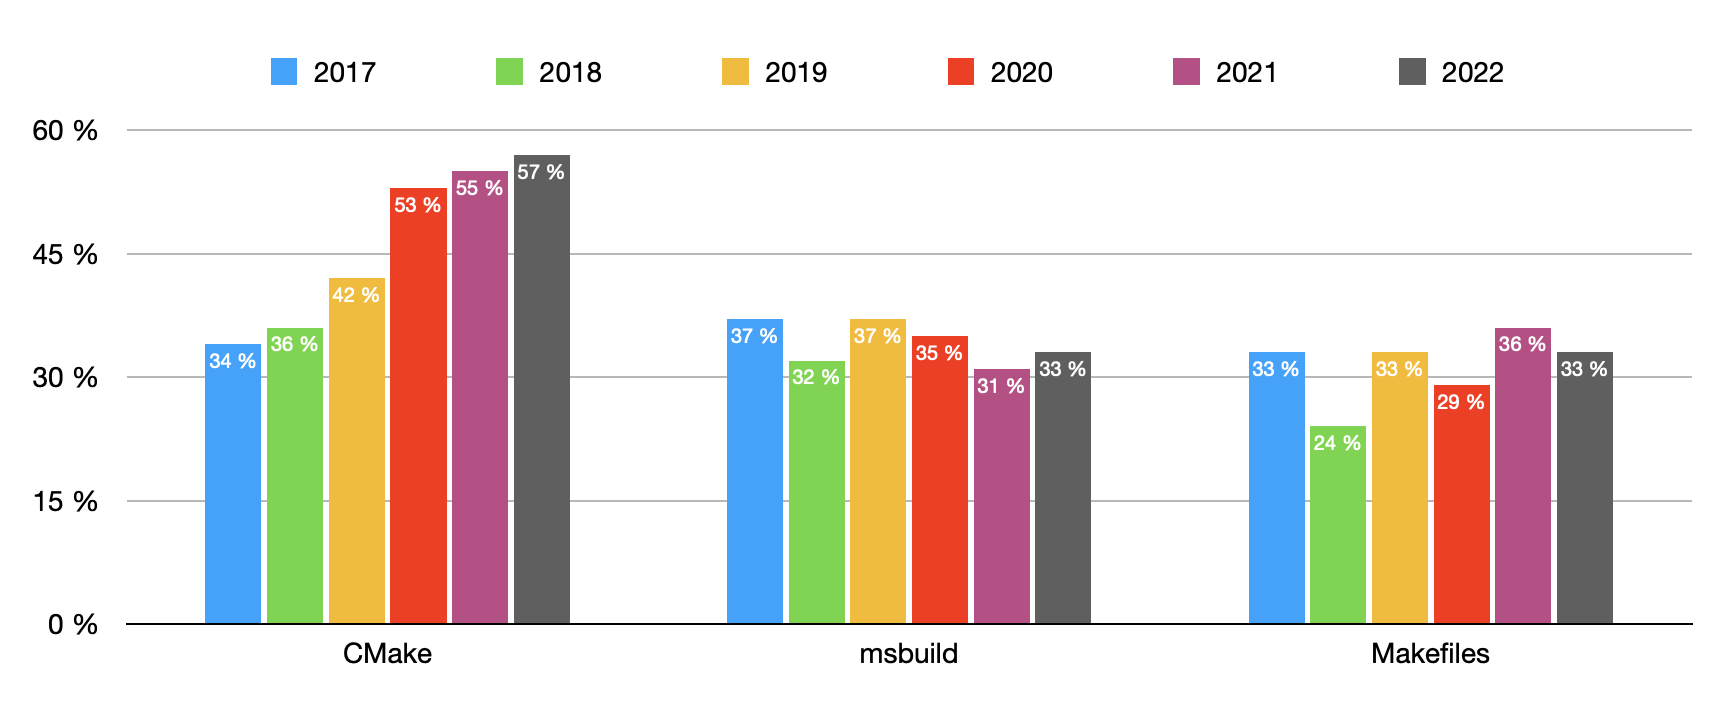
\includegraphics[width=0.65\textwidth]{cpp_build_systems}
    \caption{Comparison of the most popular build systems for \texttt{c++} projects \cite{art:cpp-build-system}}\label{fig:cpp_build_systems}
\end{figure}

Following the footsteps of the original authors, the choice fell on \textit{Bazel} \cite{repo:bazel}.
It is an open-source build system developed and maintained by Google.
It supports multiple languages and platforms and is designed to scale well with large projects, thanks to its incremental builds and caching mechanisms.

\bazel's primary goals are reproducibility and correctness, achieved by using a declarative language to define the build process and using a sandboxed environment to run the build actions.
This ensures that the build process is deterministic and that the build actions do not have side effects: all inputs and outputs must be explicitly declared for each rule.

It also features a domain-specific language \texttt{starlark} \cite{repo:starlark}, used to customize the build process even further, adding support for personalized rules and macros.
The syntax is intentionally very similar to the familiar \texttt{python}, although some more advanced language features are not included.
Custom scripts can also be shared among users, allowing the creation of packages of specialized rules for many use cases.

\subsection*{Configuration}

The \textit{Bazel} \textit{workspace} is the top-level directory.
It contains all the source files of the project, as well as scripts and configuration files.
It is defined by the presence of a \texttt{WORKSPACE.bazel} file, which specifies the project's name and is a common place to define the external dependencies.

\lstinputlisting[language=bazel,frame=single,showstringspaces=false,caption={Example of a \texttt{WORKSPACE.bazel} file},captionpos=b,label={code:workspace}]{code/example.WORKSPACE.bazel}

The project is further split into multiple \textit{packages}, each defined by a \texttt{BUILD.bazel} file.
This allows for a targeted rebuild of only the smallest subset of the dependencies when a package has been modified, using the cache for the rest.

\lstinputlisting[language=bazel,frame=single,showstringspaces=false,caption={Example of a \texttt{Build.bazel} file},captionpos=b,label={code:build}]{code/example.BUILD.bazel}

\subsection*{Dependencies}

\textit{Bazel} provides the means to manage internal and external dependencies.
This is done by downloading an archive to be included in the build process.
This step can be Simplified further by using some custom macros like \texttt{github\_archive} (\autoref{code:foreign_cc.WORKSPACE.bazel}).
The external dependencies are then built from source in a sandbox to ensure isolation and reproducibility.

Most libraries do not provide a \texttt{BUILD.bazel} file since they employ a different build system.
In those cases, it is necessary to write one manually, specifying the source files, the dependencies and the compilation flags.
To aid in the compilation, there exist several rules that ensure interoperability with the most common tools, such as \textit{CMake}, \textit{configure-make}, \textit{GNU Make}, \textit{boost}, \textit{ninja} and \textit{Meson} \cite{repo:rules-foreign-cc}.

\lstinputlisting[language=bazel,frame=single,showstringspaces=false,caption={Inclusion of the foreign_rules_cc in the WORKSPACE.bazel file},captionpos=b,label={code:foreign_cc.WORKSPACE.bazel}]{code/foreign\_cc.WORKSPACE.bazel}

The two solvers that \dlinear uses need to be included as the project's dependencies.
In the original setup, it was necessary to download the source code and compile it manually, which was a tedious process.
This step was automated by creating an ad hoc \texttt{BUILD.bazel} file for each of them, which is used when building the project and uses either \textit{cMake} and \textit{configure-make} for SoPlex and QSoptex respectively.
It also allows us to specify whether to use them as static libraries for the main executable or as dynamic libraries for the \texttt{python} bindings.

\lstinputlisting[language=bazel,frame=single,showstringspaces=false,caption={Simplified \texttt{BUILD.bazel} file for the SoPlex library},captionpos=b,label={code:soplex.BUILD.bazel}]{code/soplex.BUILD.bazel}

\bazel includes a utility that shows the project's dependency graph, which gives a good overview of the couplings between the different components.
The result is \autoref{fig:dlinear-deps}.

\begin{figure}[h]
    \centering
    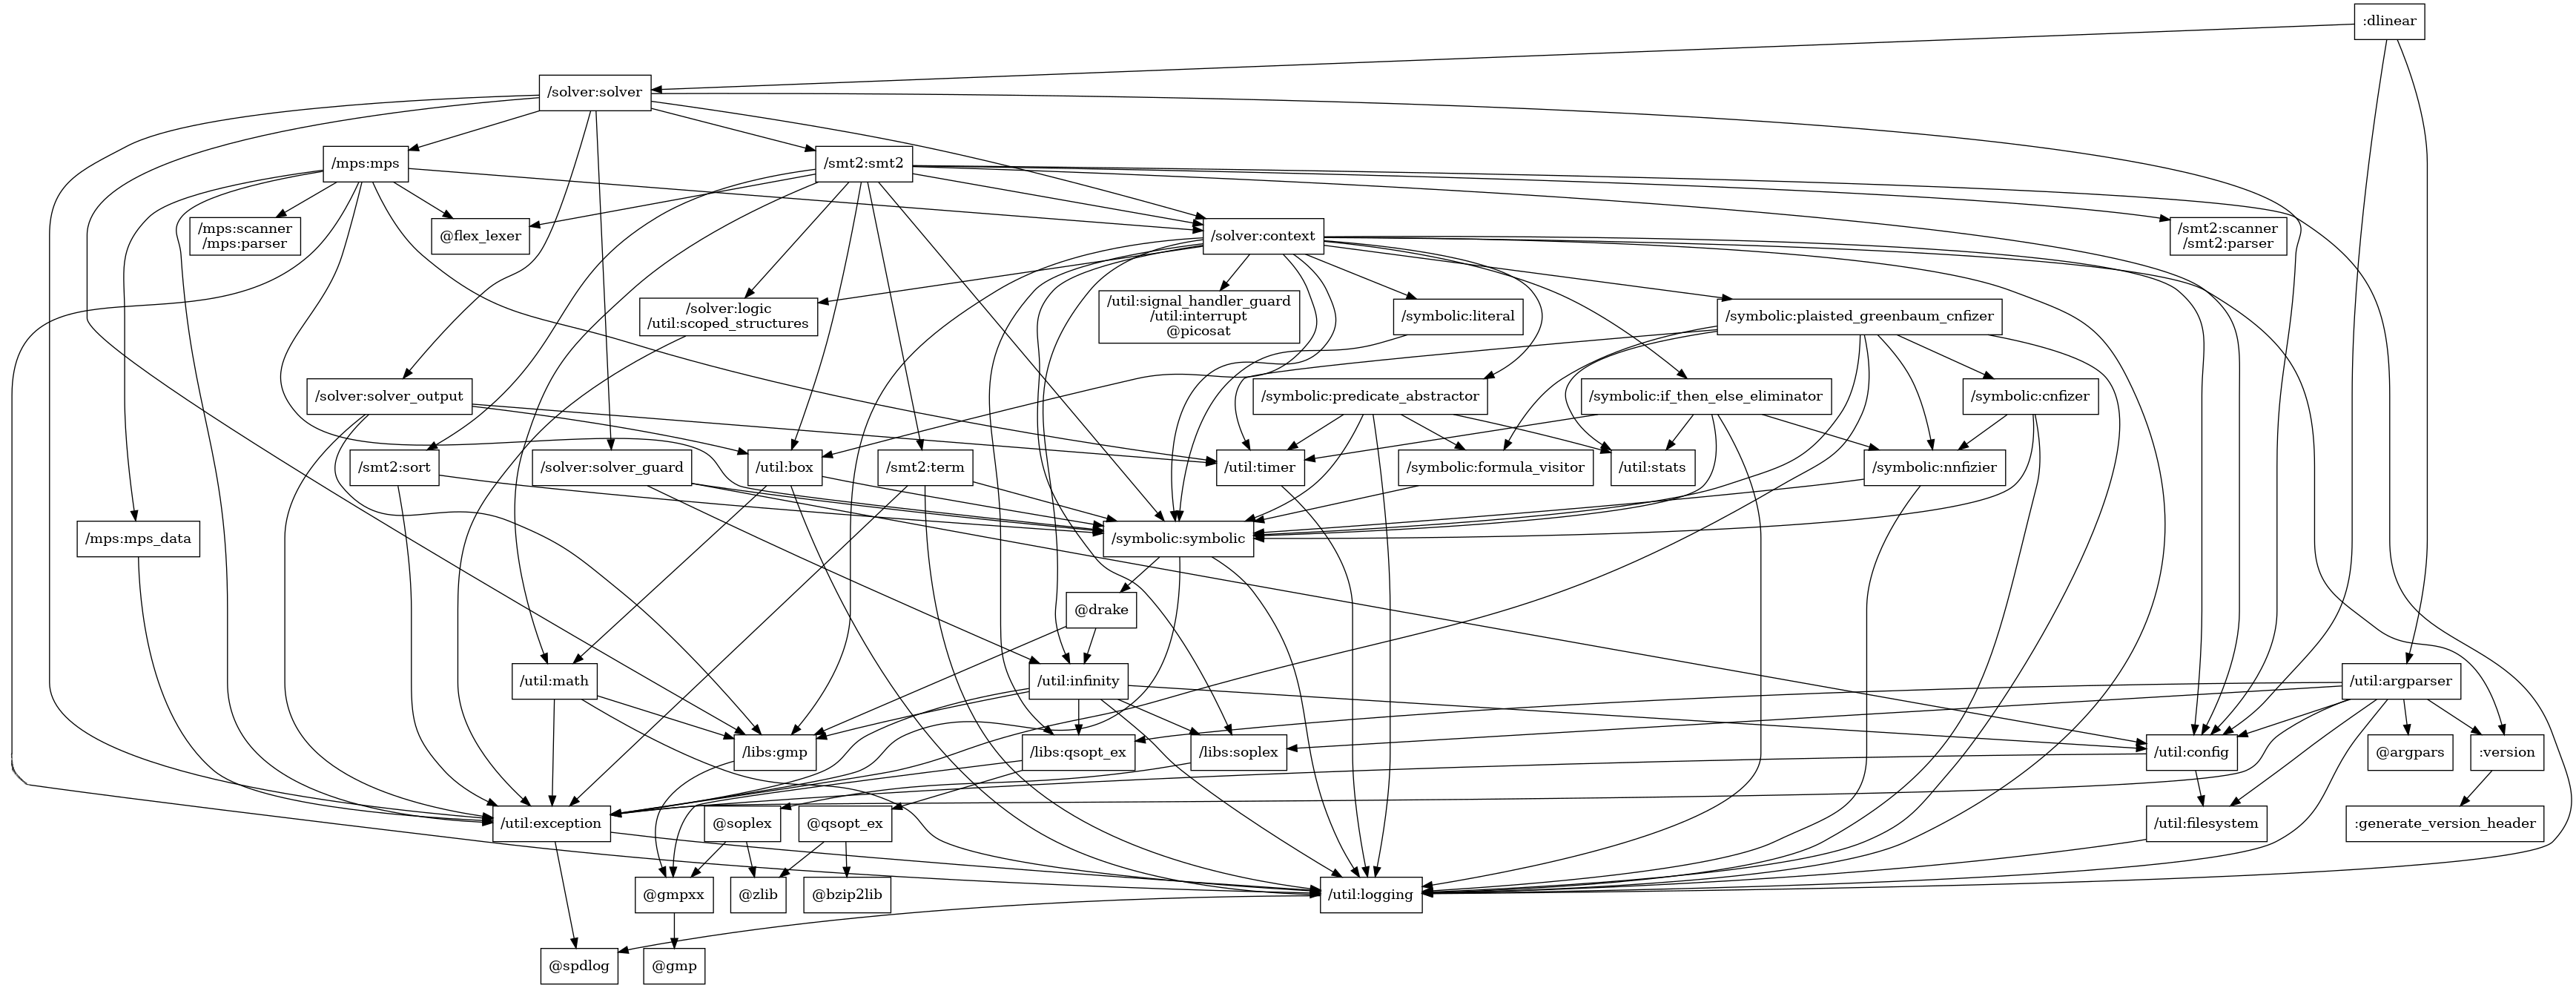
\includegraphics[width=\textwidth]{dlinear_deps}
    \caption{Visualization of the dependency graph of \dlinear as seen by \bazel}\label{fig:dlinear-deps}
\end{figure}

\chapter{Software architecture}

\section{Overview}

The software is written in \texttt{c++}, and it is formed by two main components: the \textit{dlinear library} and the \textit{python bindings}.
The project includes a \textit{benchmarking suite} and a \textit{test suite}, which are used to verify the correctness and measure the application's performance.
The \texttt{python} bindings provide a more user-friendly interface to the library and allow faster prototyping in a \texttt{python} environment.

\subsection*{Filesystem tree}

The project is organized in a structure (\autoref{fig:filesystem}) that is common to find in \texttt{bazel} projects.

The root directory contains the \texttt{WORKSPACE} file, marking the workspace's root.
The \dlinear folder contains the \texttt{c++} source code of the library.
It is further divided into subfolders, each containing the source code of a specific and primarily isolated component.
The same structure is mimicked in the \texttt{test} directory, where all the unit tests are placed.
The \pydlinear folder contains the configurations needed to create the \texttt{python} bindings and some tests to ensure their correctness. In contrast, the \texttt{benchmark} folder contains the benchmarking suite used to measure the solver's performance.

Following \texttt{bazel} conventions, the \texttt{third\_party} folder contains the external dependencies.
All the build tools and Starlark rules/macros are stored in the \texttt{tools} package.


\begin{figure}[ht]
        \begin{adjustbox}{width=0.5\textwidth,center}
                \centering
                \begin{forest}
                        pic dir tree,
                        where level=0{}{% folder icons by default; override using file for file icons
                                        directory,
                                },
                        [dlinear5
                                                [benchmark \qquad\qquad Benchmarking utilities
                                                ]
                                                [dlinear \qquad\qquad\ \ Sources
                                                                [api
                                                                ]
                                                                [libs
                                                                ]
                                                                [smt2
                                                                ]
                                                                [solver
                                                                ]
                                                                [symbolic
                                                                ]
                                                                [util
                                                                ]
                                                                [main.cpp, file
                                                                ]
                                                ]
                                                [pydlinear \qquad\qquad Python bindings
                                                                [test
                                                                ]
                                                                [pydlinear.cpp, file
                                                                ]
                                                ]
                                                [test \quad\qquad\qquad\qquad Unit tests
                                                ]
                                                [script \qquad\qquad\qquad Utility scripts
                                                ]
                                                [third\_party \qquad\quad\  External dependencies
                                                                [com_github_robotlocomotion_drake
                                                                ]
                                                ]
                                                [tools \qquad\qquad\qquad\  Build tools and Starlark macros
                                                ]
                                ]
                \end{forest}
        \end{adjustbox}
        \caption{Filesystem tree of the project}\label{fig:filesystem}
\end{figure}

\section{Design patterns}
\label{sec:patterns}

\subsection*{Pimpl idiom}

The \textit{pimpl idiom} \cite{man:pimpl} is a technique used to hide the implementation details of a class from the user.
The acronym stands for \textit{Pointer to IMPLementation}, and it is a common practice in \texttt{c++}.
The result is a reduction in compilation time upon changes in the private implementation and avoiding exposing the internal details of a class to the client (\autoref{dg:pattern-pimpl}).
This pattern can be seen as a specialization of the \textit{bridge pattern} \cite{book:gof}: the actual implementation of the class can be changed freely, decoupled from the abstraction.
The main difference is that there is usually only one concrete abstraction in the \textit{pimpl idiom}.

\plantuml{diagrams/pattern/pimpl}{Generalized UML diagram of the Pimpl idiom}{pattern-pimpl}

In \dlinear, the implementation of the solver changes drastically between \texttt{soplex} and \texttt{qsoptex}.
While the interface remains the same, the underlying implementation is chosen based on the configuration at runtime.
Therefore, the \texttt{Context} class, instantiated when the satisfiability problem needs to be verified, uses the \textit{pimpl idiom} (\autoref{dg:simplified-pimpl}).
To achieve this result, the \texttt{Context} header defines a forward declaration of the \texttt{ContextImpl} class and adds it as a private member of \texttt{Context}.
The \texttt{ContextImpl} class is then defined in its file, not exposed in the public header.
Other classes can still extend from \texttt{ContextImpl}, allowing the implementation of the solver to be changed without affecting the rest of the codebase.

\plantuml{diagrams/simplified/pimpl}{Simplified UML diagram of the implementation of the Pimpl idiom as it is used within \dlinear}{simplified-pimpl}

\subsection*{Composite and Visitor patterns}

The Composite pattern allows to treat both objects and their compositions uniformly \cite{book:gof}.
It achieves this by defining a common interface that both Leaves and Composites implement (\autoref{dg:pattern-composite}).
The approach dramatically simplifies the interaction with complex data structures, as the difference between a single object and a collection of objects is hidden.

\plantuml{diagrams/pattern/composite}{Generalized UML diagram of the Composite pattern}{pattern-composite}

The intent of the Visitor pattern is to represent an operation to be performed on the elements of an object structure.
The Visitor lets you define a new operation without changing the classes of the elements on which it operates \cite{book:gof}.
A typical application is traversing an object structure and applying an operation to each element based on its type (\autoref{dg:pattern-visitor}).
The ObjectStructure can be a simple collection or a Composite object.

\plantuml{diagrams/pattern/visitor}{Generalized UML diagram of the Visitor pattern}{pattern-visitor}

The latter is the case of \dlinear, where the \texttt{Formula} class is a Composite object, and the \texttt{FormulaVisitor} is used to traverse the structure and perform operations on each element (\autoref{dg:simplified-visitor}).
Through the Visitors, the input formula is converted in \gls{nnf}, \gls{cnf} or in a boolean formula, where each linear constraint is substituted with a boolean variable.

\plantuml{diagrams/simplified/visitor}{Simplified UML diagram of the Visitor pattern as it is used within \dlinear}{simplified-visitor}

\section{Smt2 parser}

The input files \dlinear accepts are in the format standardized by SMT-LIB \cite{docs:smtlib}.
The parser itself is generated by \texttt{bison} and \texttt{flex} and can be divided into two main parts: the lexer and the parser.
The lexer is responsible for tokenizing the input file by matching the input stream with the regular expressions defined in the \texttt{scanner.ll} file (\autoref{code:example.yy}).
The result is then fed to the parser, which uses the grammar defined in the \texttt{parser.yy} file to build an abstract syntax tree (\autoref{code:example.yy}).

Additionally, a \texttt{Driver} class coordinates the two components and provides an interface to the rest of the application, allowing it to start the parsing process and retrieve the result.
Each rule in the grammar is associated with an action, usually a \texttt{Driver}'s method call.

\lstinputlisting[language=flex,frame=single,showstringspaces=false,caption={Simplified example of a rule tokenizing the smt2 input file to reconnize the "check-sat" directive},captionpos=b,label={code:example.ll}]{code/example.ll}

\lstinputlisting[language=yacc,frame=single,showstringspaces=false,caption={Simplified example of a rule parsing the check-sat token and calling the \texttt{Driver} accordingly},captionpos=b,label={code:example.yy}]{code/example.yy}

\section{Solvers}

The two solvers supported by \dlinear are \texttt{soplex} and \texttt{qsoptex}.
Both represent the heart of the software.
They are responsible for solving the \gls{lp} part of the problem, while being directed by the \texttt{picosat} \gls{sat} solver.

While the \texttt{smt2} file is being parsed, each variable encountered is stored and added to the \texttt{Context} object.
The same is true for all the assertion regarding the constraints of the problem, which represent the theory's atoms.
When the \texttt{check-sat} directive is reached, everything comes together: the \gls{sat} solver evaluates a set of atoms that needs to be satisfied, which are then used to build the \gls{lp} problem, to be passed to either \texttt{soplex} or \texttt{qsoptex} (\autoref{dg:qsoptex}).

\plantuml{diagrams/sequence/qsoptex}{Simplified sequence diagram of the interactions between the \gls{sat} and theory solvers}{qsoptex}

\section{Python bindings}

As a programming language, \texttt{python} is widely used in the scientific community.
While its abstractions make it very easy to read and write, this comes at the expense of performance, which is usually abysmal compared to other languages, such as \texttt{c++}.
There are several \texttt{python} implementations.
The most popular one is \texttt{CPython}, which is also the one this project targets, but some alternatives include \texttt{Jython}, \texttt{IronPython} and \texttt{PyPy} \cite{man:python-implementations}.

The \texttt{CPython} implementation also allows for extensions.
The Python API defines a set of functions, macros and variables that provide access to the aspects of the Python run-time system.
To access them, it is sufficient to include the header file \texttt{Python.h}.
In other words, Python bindings (or extensions) are a way to write \texttt{c++} code that integrates seamlessly and can called from a \texttt{python} program.
Instead of using the standard \texttt{python} API, though, the much more convenient \texttt{pybind11} library is used \cite{man:pybind11}.
The main appeal of \texttt{pybind11} is that it exposes \texttt{c++} classes and functions to \texttt{python} with a very minimalistic syntax.
It also provides a rich built-in type conversion system by inferring type information using compile-time introspection.
The user can extend it even further to support custom types.

In the context of \dlinear, the main functionalities of the solver, as well as some of the most valuable data manipulation classes, have been exposed in a \texttt{python} package called, unsurprisingly, \pydlinear.
The bindings are defined in the \texttt{pydlinear.cpp} file (\autoref{code:example_python_bindings}).
The \texttt{setup.py}, with the configuration options provided by the \texttt{pyproject.toml} file, defines the steps needed for building the package to make it available to the \texttt{python} interpreter.
While the ideal scenario would be to build it on the target machine, it is possible to include a pre-build version called a \textit{wheel}.
This particular archive contains all the shared libraries that make up the package, and provided that the architecture of both the distributor's machine and the user's machine is the same, it can be used without any need for compilation by the final user.

\lstinputlisting[language=c++,frame=single,showstringspaces=false,caption={Simplified example of \pydlinear's bindings},captionpos=b,label={code:example_python_bindings}]{code/example\_python\_bindings.cpp}

The package has been uploaded to the \texttt{PyPI} repository, making it available to anyone with a \texttt{Linux x86\_64} machine and \texttt{python 3.10}.
It can be installed with the command

\begin{lstlisting}[language=bash,frame=single,showstringspaces=false]
$ pip install -i https://test.pypi.org/simple/ pydlinear==0.0.1
\end{lstlisting}
Once installed, the solver's API are accessible by importing the \pydlinear package in the script (\autoref{code:pydlinear.py}).

\lstinputlisting[language=python,frame=single,showstringspaces=false,caption={Minimal python program using \pydlinear},captionpos=b,label={code:pydlinear.py}]{code/pydlinear.py}

\section{Targets}

\bazel uses the concept of \textit{targets} to define the building blocks of a workspace.
A target can be a library, an executable, a test, a script or a data file.
What follows is a synopsis of the most essential targets used in \dlinear and their purpose.

\begin{itemize}
        \item \textbf{//dlinear}: supports both \textit{build} and \textit{run} actions.
              It is the project's main target, and it is used by the \texttt{benchmark} and \texttt{test} targets.
              It produces the fully static binary \texttt{dlinea5}, located in the \texttt{bazel-bin/dlinear} folder.
        \item \textbf{//benchmark}: supports both \textit{build} and \textit{run} actions.
              It creates a binary that wraps the \texttt{dlinear} and measures the time it takes to run the program on a set of problems with a given solver and precision.
              Both parameters can be configured using a \texttt{benchmark.conf} file.
              By default, it checks all the files in the \textit{benchmark/smt2} folder.
        \item \textbf{//test/...}: supports the \textit{test} action.
              It runs all the tests in the \dlinear.
              The logs will be saved in the \texttt{bazel-testlogs} folder.
        \item \textbf{//pydlinear}: supports the \textit{build} action.
              It creates the \texttt{pydlinear} extension.
              It can be a dependency within \bazel for other \texttt{python} targets.
\end{itemize}


% Conclusion

\chapter{Conclusions}

After a meticulous analysis of the codebase, the project has been successfully refactored.
The resulting architecture is much easier to work with, especially regarding managing and installing external dependencies, thanks to the improved integration with the \bazel build system.
The end result can be seen in the \textit{dlinear} GitHub repository \footnote{\url{https://github.com/TendTo/dlinear}}.

The tests have been extended to cover more functionalities and to be more robust, improving the software's resilience to regressions.
Finally, the benchmark framework allows for an easy and automated way to test the software's performance and gather the results using the common \texttt{csv} format.

While the final product is a perfectly functioning \gls{smt} solver, there is still much room for improvement.

First, many problems in this field are presented using the \texttt{mps} file format, which is not natively supported by the software.
This means that a conversion needs to take place before running the executable.

Furthermore, different implementations of the theory solver algorithm could be considered, such as \textit{interior-point methods}.
They are more suitable for parallelization and can outperform the simplex approach, provided the problem is enormous and it is possible to exploit specific structures, often represented as nested sets of blocks in a tree-like structure \cite{paper:parallel-interior-point}.
Switching to the interior-point method could be beneficial when it would lead to a faster solution.
However, the decision would probably require some form of input analysis, with the cost that this entails.

Once all the issues have been addressed, more complete documentation will need to be produced to allow for a more straightforward approach for interested newcomers.

I hope I will have the chance to mark all these points as done in the future.


% Bibliography
\printglossary
\pagebreak
\printbibliography
\pagebreak

\begin{appendices}
    \chapter{Benchmarks}\label{appendix:benchmarks}
    The problems used in the benchmarks are comprised of samples from:

    \begin{itemize}
        \item Csaba Mészáros LP collection  \footnote{\url{http://old.sztaki.hu/~meszaros/public_ftp/lptestset/}}
        \item the Netlib LP tests, including the kennington tests \footnote{\url{http://www.netlib.org/lp/data/}}
        \item Hans Mittelmann's benchmark instances \footnote{\url{https://plato.asu.edu/ftp/lptestset/}}
    \end{itemize}
    The benchmarking suite has been run on a machine with the following specifications.
    Each run utilized only one core.

    \begin{itemize}
        \item 2 Intel Xeon E5-2699 v4 processors (2.2 GHz, 22 cores, 55 MB cache)
        \item 44 cores (2 processors * 22 cores), totalling 4840 across the standard nodes
        \item 128 GB memory - (8 DDR4 RDIMMs, each with 16GB) - ie. 2.9 GB per core
    \end{itemize}
    The results were then filtered only to include runs in which at least one solver took longer than 10 seconds to output the result.
    Legend:

    \begin{itemize}
        \item \textbf{File}: the name of the file used for the benchmark.
        \item \textbf{Solver}: the solver used for the benchmark. It can be either \texttt{soplex} or \texttt{qsoptex}.
        \item \textbf{\#a}: the number of assertions contained within the file.
        \item \textbf{Result}: the result of the benchmark. It can be either \textit{delta-sat} or \textit{unsat}.
        \item \textbf{$\delta_i$}: the precision that was given to the solver.
        \item \textbf{$\delta_a$}: the achieved precision of the solver.
        \item \textbf{Time}: the time needed to solve the file in seconds.
    \end{itemize}

    % \subsection*{QF_LRA}

    % \begin{longtable}{l|ll|lll|lll}
    %     \hline
    %                    &                      &               & \multicolumn{3}{c}{QSoptex} & \multicolumn{3}{c}{Soplex}                                                                                 \\
    %     \bfseries File & \bfseries $\delta_i$ & \bfseries \#a & \bfseries $\delta_a$        & \bfseries Time             & \bfseries Result & \bfseries $\delta_a$ & \bfseries Time & \bfseries Result   \\
    %     \hline
    %     \endhead
    %     \csvreader[head to column names]{data/smtbenchmark.csv}{}
    %     {                                                                                                                                                                                                \\
    %     \file          & \precision           & \assertions   & \actualPrecisionQ           & \timeQ                     & \resultQ         & \actualPrecisionS    & \timeS         & \resultS         }
    % \end{longtable}

    \subsection*{LP}

    \begin{longtable}{l|ll|lll|lll}
        \hline
                       &                      &               & \multicolumn{3}{c}{QSoptex} & \multicolumn{3}{c}{Soplex}                                                                                 \\
        \bfseries File & \bfseries $\delta_i$ & \bfseries \#a & \bfseries $\delta_a$        & \bfseries Time             & \bfseries Result & \bfseries $\delta_a$ & \bfseries Time & \bfseries Result   \\
        \hline
        \endhead
        \csvreader[head to column names]{data/lpbenchmark.csv}{}
        {                                                                                                                                                                                                \\
        \file          & \precision           & \assertions   & \actualPrecisionQ           & \timeQ                     & \resultQ         & \actualPrecisionS    & \timeS         & \resultS         }
    \end{longtable}

    % \subsection*{Sloane-Stufken}

    % \begin{longtable}{lllll|ll|lll|lll}
    %     \hline
    %                  &              &              &              &             &                      &               & \multicolumn{3}{c}{QSoptex} & \multicolumn{3}{c}{Soplex}                                                                                 \\
    %     \bfseries s1 & \bfseries k1 & \bfseries s2 & \bfseries k2 & \bfseries t & \bfseries $\delta_i$ & \bfseries \#a & \bfseries $\delta_a$        & \bfseries Time             & \bfseries Result & \bfseries $\delta_a$ & \bfseries Time & \bfseries Result   \\
    %     \hline
    %     \endhead
    %     \csvreader[head to column names]{data/ssbenchmark.csv}{}
    %     {                                                                                                                                                                                                                                                         \\
    %     \si          & \ki          & \sii         & \kii         & \t          & \precision           & \assertions   & \actualPrecisionQ           & \timeQ                     & \resultQ         & \actualPrecisionS    & \timeS         & \resultS         }
    % \end{longtable}

    \chapter{Detailed UML diagrams}

    The following are the same diagrams described in \autoref{sec:patterns} but with more details.

    \plantuml[1.2]{diagrams/dlinear/pimpl}{UML class diagram of the Pimpl pattern as it is used in \dlinear.\\It describes the \texttt{Context} class, that provides an abstraction over the \gls{sat} and theory solvers' implementations}{dlinear-pimpl}

    \plantuml[1.3]{diagrams/dlinear/visitor}{UML class diagram of the visitor pattern as it is used in \dlinear.\\It describes the \texttt{FormulaVisitor} family of classes, used in the conversion of formulas in a valid \gls{cnf}}{dlinear-visitor}

    \chapter{Program usage}

    The \dlinear executable built by \bazel using the \texttt{bazel build //dlinear} command will be placed in the \texttt{bazel-bin/dlinear} directory.
    Sine the binary is statically linked by default, it can be moved to any destination without problems.
    The following is the output obtained by running \dlinear with the \texttt{--help} flag.
    It lists all the options available to the user.

    \lstinputlisting[basicstyle=\tiny,language=bash,frame=single,showstringspaces=false,caption={Output using the \texttt{--help} flag},captionpos=b,label={code:help}]{code/help}

\end{appendices}


\end{document}
